\chapter{Document Retrieval}

We are given a collection $D' = \{d_1, \ldots, d_{N-1}\}$ of documents. Each of $d_i$ is a string over an alphabet $\Sigma' = [2,\sigma]$ terminated by a sentinel symbol $1$ (or \#). We define $D = D' \cup d_0$ with a sentinel document $d_0 = 0$. We now want to answer word queries $Q = \{q_0, \ldots, q_{m-1}\}$. $Q$ is called \defi{bag of words}{Bag of Words} and is an unordered set of size $m$.

\begin{Definition}
  Given a collection $D$, a query $Q$ of length $m$ and a similarity measure $\mathcal{S} : D \times \mathcal{P}_{=m}(\Sigma') \to \mathbb{R}$. Calculate the \defi{top-k documents}{Top-k Documents} of $D$ with regard to $Q$ an $\mathcal{S}$.\newline
  That is a sorted list $T = \{\tau_0, \ldots, \tau_{k-1}\}$ with $\mathcal{S}(d_{\tau_i}, Q) \geq \mathcal{S}(d_{\tau_{i + 1}}, Q)$ for $0 \leq i < k$ and $\mathcal{S}(d_{\tau_{k-1}},Q) \geq \mathcal{S}(d_j, Q)$ for $j \not\in T$.
\end{Definition}

\section{Similarity Measures}

\begin{Definition}
  The following document dependent factors appear in many different similarity measures~$\mathcal{S}$:
  \begin{itemize}
    \item $f_{d,q}$ is the \defi{term frequency}{Term Frequency}. It counts the number of times, word $q$ appears in document~$d$.
    \item $F_{D,q}$ is the \defi{document frequency}{Document Frequency}. It counts the number of distinct documents from~$D$ containing~$q$ at least once.
  \end{itemize}
\end{Definition}

\begin{Definition}
  The \defi{Okapi BM25}{Okapi BM25} similarity measure is given by:
  \begin{align}
    \mathcal{S}_{Q,d}^{BM25} = \sum\limits_{q \in Q}
    \frac{\left(k_1 + 1\right)f_{d,q}}{k_1\left(1 - b + \frac{n_d}{n_{avg}}\right) + f_{d,q}}
    \cdot f_{Q,q} \cdot
    \ln\frac{N - F_{D,q} + 0.5}{F_{D,q} + 0.5}
  \end{align}
  Here $n_d$ is the length of document $d$ and $n_{avg}$ is the average document length.
\end{Definition}

There are several other possible ideas to build a similarity measure:
\begin{itemize}
  \item Documents can be assigned \defi{static weights}{Static Weighting}. An example is the Page-Rank algorithm.
  \item A \defi{language model}{Language Model} can be used to compute the probability to generate the query using the text statistics of each document.
  \item In a \defi{vector space model}{Vector Space Model} we compute the cosine of the angle in $\sigma$-dimensional space between a query vector and a document vector.
  \item \defi{Zone ranking}{Zone Ranking} weighs words appearing in the title of a web page weigh more than words in the body.
\end{itemize}

\section{Inverted Index}

\begin{Definition}
  In an \defi{inverted index}{Inverted Index} (IVI) for each term $q$ (excluding the sentinels) a list of pairs of document id and term frequency is stored. The pairs are ordered according to their document ids. Further for each term the document frequency is stored.
\end{Definition}

To process a query we sequentially iterate through the lists containing the query phrases and calculate the ranking function. The query complexity therefore depends on the document frequency.

It is not possible to answer phrase queries with this variant of an inverted index. Direct support of arbitrary phrase queries would require $\mathcal{O}(n^2)$ lists.

\begin{Example}
  Consider the three documents $\mathcal{D} = \{d_1, d_2, d_3\}$:
  \begin{align*}
    d_1 &: \text{is big data really big} \\
    d_2 &: \text{is it big in science} \\
    d_3 &: \text{big data is big}
  \end{align*}
  We will get the following inverted index:
  \begin{align*}
    \text{big} &: \{(1,2), (2,1), (3,2)\}  & F_{\mathcal{D}, \text{big}} = 3 \\
    \text{data} &: \{(1,1), (3,1)\} & F_{\mathcal{D}, \text{data}} = 2 \\
    \text{in} &: \{(2,1)\} & F_{\mathcal{D}, \text{in}} = 1 \\
    \text{is} &: \{(1,1), (2,1), (3,1)\} & F_{\mathcal{D}, \text{is}} = 3 \\
    \text{really} &: \{(1,1)\} & F_{\mathcal{D}, \text{really}} = 1 \\
    \text{science} &: \{(2,1)\} & F_{\mathcal{D}, \text{science}} = 1
  \end{align*}
\end{Example}

\begin{Theorem}
  An inverted index can be represented in $n\mathcal{H}_0(\mathcal{D}) + 3n + o(n) + \mathcal{O}(\sigma \log n)$ bits, where $n = \sum_{d \in \mathcal{D}} n_d$ and $f_{\mathcal{D},q} = \sum_{d \in \mathcal{D}} f_{d,q}$.
\end{Theorem}

\begin{Proof}
  For each term we use Elias-Fano-Encoding to store the increasing list of document ids. The list of frequencies itself is unary encoded decreased by one (each frequency~$x$ is encoded by~$x$ bits). With this representation we get:
  \begin{align}
    \begin{aligned}
      \proc{Space(IVI)}
      &\stackrel{\mathclap{\text{\ref{def:eliasDeltaEncoding}}}}{=}
      \sum\limits_{q \in \Sigma}
      \underbrace{2F_{\mathcal{D},q} + F_{\mathcal{D},q} \log\frac{N}{F_{\mathcal{D}, q}} + o(F_{\mathcal{D},q})}_{\text{document ids}} +
      \underbrace{f_{\mathcal{D},q}}_{\text{frequencies}} +
      \underbrace{\mathcal{O}(\log n)}_{\text{pointer}} \\
      &\leq 3n + o(n) + \mathcal{O}(\sigma \log n) + \sum\limits_{q \in \Sigma} F_{\mathcal{D},q}\log\frac{n}{F_{\mathcal{D},q}} \\
      &\stackrel{\mathclap{(*)}}{\leq}
      3n + o(n) + \mathcal{O}(\sigma \log n) +
      n\sum\limits_{q \in \Sigma}\frac{f_{\mathcal{D},q}}{n}\log\frac{n}{f_{\mathcal{D},q}} \\
      &= n\mathcal{H}_0(\mathcal{D}) + 3n + o(n) + \mathcal{O}(\sigma \log n)
    \end{aligned}
  \end{align}
  In $(*)$ we assumed that $f_{\mathcal{D},q} < \frac{n}{2}$ for all $q$. When the inverted index contains a sufficient amount of documents, this is safe to assume.
\end{Proof}

\section{GREEDY framework}

\begin{Definition}
  Let $\mathcal{D}$ be the \defi{document array}{Document Array} of length $n$. For each suffix $\id{SA}[i]$ the document array $\mathcal{D}[i]$ contains the identifier of the document, in which suffix $\id{SA}[i]$ starts. A suffix array (or suffix tree) with this information added is called \defi{generalized suffix array}{Generalized Suffix Array} (or \defi{generalized suffix tree}{Generalized Suffix Tree}).
\end{Definition}

\begin{Definition}
  The \defi{GREEDY framework}{GREEDY Framework} for single term $f_{d,q}$-ranking of Culpepper et al. \cite{Culpepper2010} consists of:
  \begin{itemize}
    \item A compressed suffix array \id{CSA} of concatenation $\mathcal{D}$.
    \item A wavelet tree of the document array of $D$.
  \end{itemize}
\end{Definition}

\section{Document Frequency $F_{\mathcal{D},q}$}

In this section we will see how to efficiently compute the document frequency $F_{\mathcal{D},q}$ for a given query $q$ following a method from Sadakane \cite{Sadakane2007}.

\begin{Definition}
  The \defi{binary generalized suffix tree}{Binary Generalized Suffix Tree} (\id{BGST}) of a text is the suffix tree with inserted inner nodes, such that the each vertex has degree $0$ or $2$. Figure~\ref{fig:binaryGeneralizedSuffixTreeExample} shows the \id{BGST} for \texttt{LA O LA \# O LA LA LA \# O O LA \# \$}.
\end{Definition}

To count the document frequency $F_{\mathcal{D},q}$, execute the following steps:
\begin{enumerate}
  \item Build the \id{BGST}.
  \item For each inner node $v$ in \id{BGST} keep a list $L_v$ of repeated documents. A document $d$ is added to $L_v$, if $d$ occurs in a leaf of the left and of the right subtree.
  \item For a pattern $q$ let $v_q$ be the \defi{locus}{Locus}, that is the lowest node which path is prefixed by $q$. $F_{\mathcal{D},q}$ equals the number of leaves in the subtree of $v_q$ minus the number of repeated documents ($\sum_{v \in T_{v_q}} \vert L_v \vert$) in $v_q$'s subtree $T_{v_q}$.
\end{enumerate}
To find the number of repeated documents in the subtree of an inner node, number the nodes in order (as in Figure~\ref{fig:binaryGeneralizedSuffixTreeExample}). Traverse in this order and append $\vert L_v \vert$ in unary coding ($\vert L_v \vert$ $0$s and one $1$) to a bitvector $H$, which was initialized with a single $1$. Then all nodes of each possible subtree are contiguous and the number of repeated documents can be calculated by two select queries. This is shown in Algorithm~\ref{alg:documentFrequency}. The runtime depends only on the time to do the backward search.

\begin{figure}[htb]
  \centering
  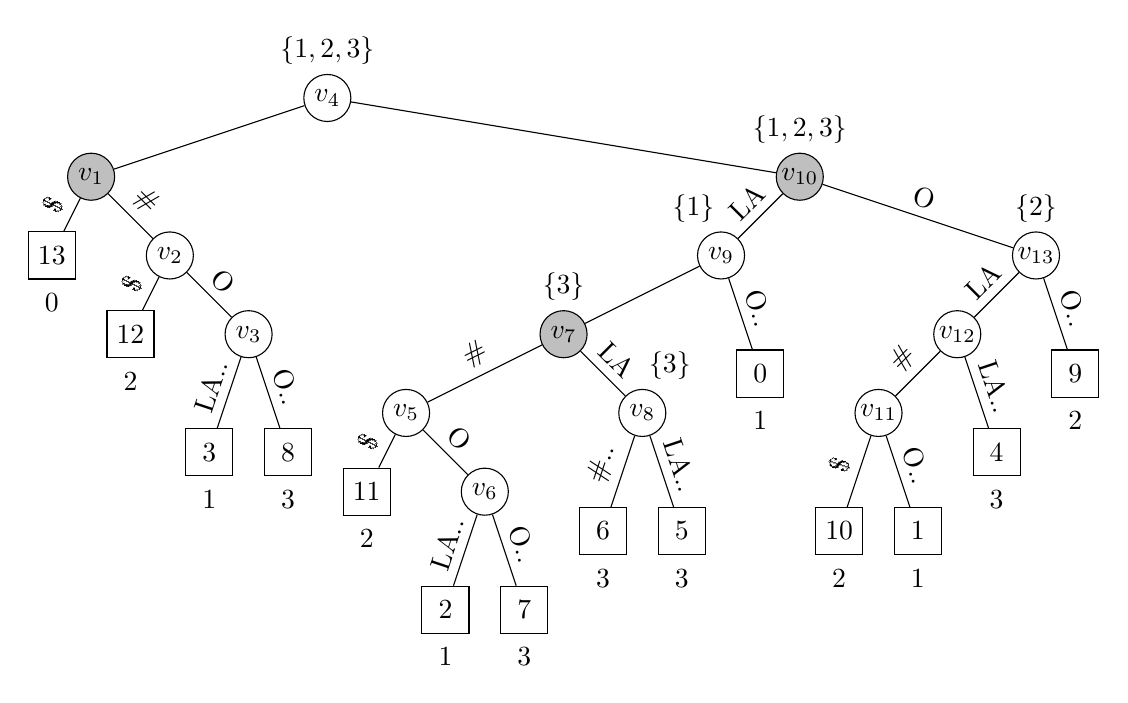
\begin{tikzpicture}[x={(5mm, 0mm)}]
  \tikzstyle{vertex}=[draw,minimum size=17pt, inner sep=0pt]
  \node[vertex, circle] (v4) at (0, 0) {$v_4$};
  \node (l4) at (0, 0.6) {$\{1,2,3\}$};

  \node[vertex, circle, fill=lightgray] (v1) at (-6, -1) {$v_1$};
  \draw (v4) -- (v1);

  \node[vertex, circle] (v2) at (-4, -2) {$v_2$};
  \draw (v1) -- (v2) node[above, sloped, pos=0.5] {\#};

  \node[vertex, circle] (v3) at (-2, -3) {$v_3$};
  \draw (v2) -- (v3) node[above, sloped, pos=0.5] {O};

  \node[vertex, circle, fill=lightgray] (v10) at (12, -1) {$v_{10}$};
  \node (l10) at (12, -0.4) {$\{1,2,3\}$};
  \draw (v4) -- (v10);

  \node[vertex, circle] (v9) at (10, -2) {$v_9$};
  \node (l9) at (9.3, -1.4) {$\{1\}$};
  \draw (v10) -- (v9) node[above, sloped, pos=0.5] {LA};

  \node[vertex, circle, fill=lightgray] (v7) at (6, -3) {$v_7$};
  \node (l7) at (6, -2.4) {$\{3\}$};
  \draw (v9) -- (v7);

  \node[vertex, circle] (v5) at (2, -4) {$v_5$};
  \draw (v7) -- (v5) node[above, sloped, pos=0.5] {\#};

  \node[vertex, circle] (v6) at (4, -5) {$v_6$};
  \draw (v5) -- (v6) node[above, sloped, pos=0.5] {O};

  \node[vertex, circle] (v8) at (8, -4) {$v_8$};
  \node (l8) at (8.7, -3.4) {$\{3\}$};
  \draw (v7) -- (v8) node[above, sloped, pos=0.5] {LA};

  \node[vertex, circle] (v13) at (18, -2) {$v_{13}$};
  \node (l13) at (18, -1.4) {$\{2\}$};
  \draw (v10) -- (v13) node[above, sloped, pos=0.5] {O};

  \node[vertex, circle] (v12) at (16, -3) {$v_{12}$};
  \draw (v13) -- (v12) node[above, sloped, pos=0.5] {LA};

  \node[vertex, circle] (v11) at (14, -4) {$v_{11}$};
  \draw (v12) -- (v11) node[above, sloped, pos=0.5] {\#};

  \node[vertex] (s13) at (-7, -2) {$13$};
  \node (d13) at (-7, -2.6) {$0$};
  \draw (v1) -- (s13) node[above, sloped, pos=0.5] {\$};

  \node[vertex] (s12) at (-5, -3) {$12$};
  \node (d12) at (-5, -3.6) {$2$};
  \draw (v2) -- (s12) node[above, sloped, pos=0.5] {\$};

  \node[vertex] (s3) at (-3, -4.5) {$3$};
  \node (d3) at (-3, -5.1) {$1$};
  \draw (v3) -- (s3) node[above, sloped, pos=0.5] {LA..};

  \node[vertex] (s8) at (-1, -4.5) {$8$};
  \node (d8) at (-1, -5.1) {$3$};
  \draw (v3) -- (s8) node[above, sloped, pos=0.5] {O..};

  \node[vertex] (s11) at (1, -5) {$11$};
  \node (d11) at (1, -5.6) {$2$};
  \draw (v5) -- (s11) node[above, sloped, pos=0.5] {\$};

  \node[vertex] (s2) at (3, -6.5) {$2$};
  \node (d2) at (3, -7.1) {$1$};
  \draw (v6) -- (s2) node[above, sloped, pos=0.5] {LA..};

  \node[vertex] (s7) at (5, -6.5) {$7$};
  \node (d7) at (5, -7.1) {$3$};
  \draw (v6) -- (s7) node[above, sloped, pos=0.5] {O..};

  \node[vertex] (s6) at (7, -5.5) {$6$};
  \node (d6) at (7, -6.1) {$3$};
  \draw (v8) -- (s6) node[above, sloped, pos=0.5] {\#..};

  \node[vertex] (s5) at (9, -5.5) {$5$};
  \node (d5) at (9, -6.1) {$3$};
  \draw (v8) -- (s5) node[above, sloped, pos=0.5] {LA..};

  \node[vertex] (s0) at (11, -3.5) {$0$};
  \node (d0) at (11, -4.1) {$1$};
  \draw (v9) -- (s0) node[above, sloped, pos=0.5] {O..};

  \node[vertex] (s9) at (19, -3.5) {$9$};
  \node (d9) at (19, -4.1) {$2$};
  \draw (v13) -- (s9) node[above, sloped, pos=0.5] {O..};

  \node[vertex] (s4) at (17, -4.5) {$4$};
  \node (d4) at (17, -5.1) {$3$};
  \draw (v12) -- (s4) node[above, sloped, pos=0.5] {LA..};

  \node[vertex] (s10) at (13, -5.5) {$10$};
  \node (d10) at (13, -6.1) {$2$};
  \draw (v11) -- (s10) node[above, sloped, pos=0.5] {\$};

  \node[vertex] (s1) at (15, -5.5) {$1$};
  \node (d1) at (15, -6.1) {$1$};
  \draw (v11) -- (s1) node[above, sloped, pos=0.5] {O..};
\end{tikzpicture}

  \caption{The binary generalized suffix tree of an example document collection $\mathcal{D} = \texttt{LA O LA \# O LA LA LA \# O O LA \# \$}$. The filled vertices are the dummy nodes added to get a binary tree. Round nodes are inner nodes, square nodes are leaves corresponding to suffixes. The number below each leaf is the entry in the document array.}
  \label{fig:binaryGeneralizedSuffixTreeExample}
\end{figure}

\begin{algorithm}[htb]
  \begin{codebox}
    \Procname{$\proc{Document-Frequency}(q)$}
    \li $[l,r] \gets \proc{Backward-Search(\id{CSA}, q)}$
    \li $s \gets r - l + 1$
    \li $y \gets \proc{Select}_1(r, H)$
    \li \If $l \isequal 0$
        \Then
    \li   \Return $s - (y - r + 1)$
    \li \Else
    \li   $x \gets \proc{Select}_1(l, H)$
    \li   \Return $s - (y - r + 1 - (x - l + 1))$
        \End
  \end{codebox}
  \caption{Compute the document frequency $F_{\mathcal{D},q}$ for query $q$.}
  \label{alg:documentFrequency}
\end{algorithm}

\begin{Example}
  Figure~\ref{fig:binaryGeneralizedSuffixTreeExample} shows the \id{BGST} for \texttt{LA O LA \# O LA LA LA \# O O LA \# \$}. We get the following bitvector $H$:
  \begin{align*}
    H = 1
    \underbrace{1}_{v_1}
    \underbrace{1}_{v_2}
    \underbrace{1}_{v_3}
    \underbrace{0001}_{v_4}
    \underbrace{1}_{v_5}
    \underbrace{1}_{v_6}
    \underbrace{01}_{v_7}
    \underbrace{01}_{v_8}
    \underbrace{01}_{v_9}
    \underbrace{0001}_{v_{10}}
    \underbrace{1}_{v_{11}}
    \underbrace{1}_{v_{12}}
    \underbrace{01}_{v_{13}}
  \end{align*}
  Let's now consider $q = \texttt{LA}$. Then \proc{Backward-Search} returns suffix array interval $[4,9]$. Executing the steps in Algorithm~\ref{alg:documentFrequency} yields $s = 6$, $y = 15$ and $x = 7$, so that $3$ is returned.
\end{Example}

\begin{Theorem}
  The document frequency can be calculated with an index needing $\mathcal{O}(n + \vert \id{CSA} \vert)$ bits space.
\end{Theorem}

\begin{Proof}
  The bitvector $H$ has maximum size $2n - N$. Additionally $o(n)$ bits for a constant time select structure are needed. The only thing left is the space needed for \id{CSA}.
\end{Proof}

\subsection{Calculating $F_{\mathcal{D}_v, q}$}

Let $F_{\mathcal{D}_v, q}$ be the subset of documents which are represented by a node in the wavelet tree over the document array. To compute it efficiently we introduce another array:

\begin{Definition}
  The \defi{repetition array}{Repetition Array} $R$ contains for each $0$ in $H$ the corresponding repeated element of the associated node.
\end{Definition}

We can build a wavelet tree \id{WTD} over the document array and a wavelet tree \id{WTR} over the repetition array. Using $\proc{Select}_1$ we can as above convert an interval $[l,r]$ of the suffix array into ranges in the two wavelet trees. When traversing \id{WTD} we can simultaneously traverse \id{WTR}. The size of the range in \id{WTR} always counts the number of repetitions.

\begin{Example}
  Continuing above example, we get for $H$ and $R$:
  \begin{align*}
    H &= 1
    \underbrace{1}_{v_1}
    \underbrace{1}_{v_2}
    \underbrace{1}_{v_3}
    \underbrace{0001}_{v_4}
    \underbrace{1}_{v_5}
    \underbrace{1}_{v_6}
    \underbrace{01}_{v_7}
    \underbrace{01}_{v_8}
    \underbrace{01}_{v_9}
    \underbrace{0001}_{v_{10}}
    \underbrace{1}_{v_{11}}
    \underbrace{1}_{v_{12}}
    \underbrace{01}_{v_{13}} \\
    R &=
    \underbrace{123}_{v_4}
    \underbrace{3}_{v_2}
    \underbrace{3}_{v_8}
    \underbrace{1}_{v_9}
    \underbrace{123}_{v_{10}}
    \underbrace{2}_{v_{13}}
  \end{align*}
\end{Example}

